\section{Synthetic Data Generation Pipeline (\texttt{data-gen})}
As the repository expands to include other projects (such as neural networks for anomaly detection), this section specifically details the anomaly generation pipeline.

\subsection{File Structure Review}
The repository enforces a strict separation of concerns, divided into modular directories:

\begin{itemize}
    \item \textbf{\texttt{data-gen/data/}}: Contains raw background sensor readings (e.g., \texttt{2015\_months\_DebitDoseA.txt}) used as a real-world baseline, along with generated output datasets and the class mapping file (\texttt{class\_mapping.txt}).
    \item \textbf{\texttt{data-gen/anomalies/}}: Contains the normalized \texttt{.csv} blueprints (templates) for the 6 anomaly shapes: \texttt{bell}, \texttt{bell\_sq}, \texttt{fast\_ascend}, \texttt{fast\_descend}, \texttt{M}, and \texttt{square}.
    \item \textbf{\texttt{data-gen/src/}}: Stores the pure mathematical generator library (\texttt{anomaly\_generator.py}), decoupled from direct script logic.
    \item \textbf{\texttt{data-gen/script/}}: Stores execution pipelines, real-data evaluators, and visualization launchers. Scripts utilize the math from \texttt{data-gen/src/} to generate datasets or debug plots.
    \item \textbf{\texttt{data-gen/logs/}}: The destination for Plotly's interactive HTML visualizations and PNG exports.
\end{itemize}

\subsection{Explanation of the Engine and Scripts}

\subsubsection{\texttt{data-gen/src/anomaly\_generator.py}}
This is the core computational engine. It provides the \texttt{generate\_anomaly()} function which transforms a normalized CSV blueprint into a physical discrete array. The engine mathematically scales the template temporally (period span) and vertically (amplitude intensity) while embedding Gaussian deformation using the limits declared in the CSV file.

\subsubsection{\texttt{data-gen/script/evaluate\_real\_data.py}}
This script analyzes the original physical gamma sensor data to extract baseline drift and noise characteristics. It calculates the moving average baseline to isolate high-frequency noise from the slow, low-frequency sensor drift. Crucially, it calculates the volatility $\sigma$ of the Ornstein-Uhlenbeck (OU) process used for synthetic generation. Because a moving average heavily dampens step-by-step differences, the script applies a calibrated mathematical correction to $\sigma$ (e.g., $0.037$) so that the synthetic baseline explores the same dynamic range (15-27 units over 40,000 points) as the real 2015 sensors. The results are saved to \texttt{real\_data\_params.json}.

\subsubsection{\texttt{data-gen/script/interactive\_labeling\_helper.py}}
An interactive visualization tool that plots the real, unlabelled sensor data alongside its calculated baseline and a $3\sigma$ confidence threshold. It allows the user to hover over visual anomalies in the real data to measure their exact amplitude and period, which directly informs the configuration parameters for synthetic generation.

\subsubsection{\texttt{data-gen/script/generate\_custom\_dataset.py}}
The primary execution pipeline for training data. It utilizes a centralized \texttt{CONFIG} dictionary explicitly defining generation constraints (such as anomaly amplitude, period, and frequency) and seamlessly imports the real-world statistical parameters generated by \texttt{evaluate\_real\_data.py}. 

Spanning datasets of up to 10,000,000 steps, it generates a highly realistic \textbf{wandering baseline} using a chunk-by-chunk OU process overlaid with high-frequency Gaussian noise. It randomly samples anomaly templates from the library, calculates randomized injection amplitudes and duration bounds, and injects them into the signal. Each injected shape is mapped to a unique multi-class integer ID, tagging absolute ground-truth labels alongside the continuous signal.

\begin{figure}[H]
    \centering
    
\includegraphics[width=0.7\textwidth]{media/synthetic_custom_dataset.png}
    \caption{Output of generate\_custom\_dataset.py}
\end{figure}

\subsubsection{\texttt{data-gen/script/test\_generator\_deformation.py}}
A visual sandbox and boundary debugging tool. Iterating automatically over all discovered templates in the \texttt{data-gen/anomalies/} directory, it runs exactly 5 generation iterations of each template to visually verify and validate the variability limits enforced by the template's deformation parameters. Exports directly to HTML and PNG.

\subsubsection{\texttt{data-gen/script/visualize\_anomalies\_templates.py}}
This script visualizes the pure original mathematical blueprints. It renders the shapes and their interpolation properties exactly as described in the blueprint CSV, without injecting randomization or temporal noise.

\begin{figure}[p]
    \centering
    \begin{minipage}[c]{0.46\textwidth}
        \centering
        
\includegraphics[width=\linewidth,height=0.85\textheight,keepaspectratio]{media/anomaly_templates.png}
        \caption{Output of visualize\_anomalies\_templates.py}
    \end{minipage}\hfill
    \begin{minipage}[c]{0.5\textwidth}
        \centering
        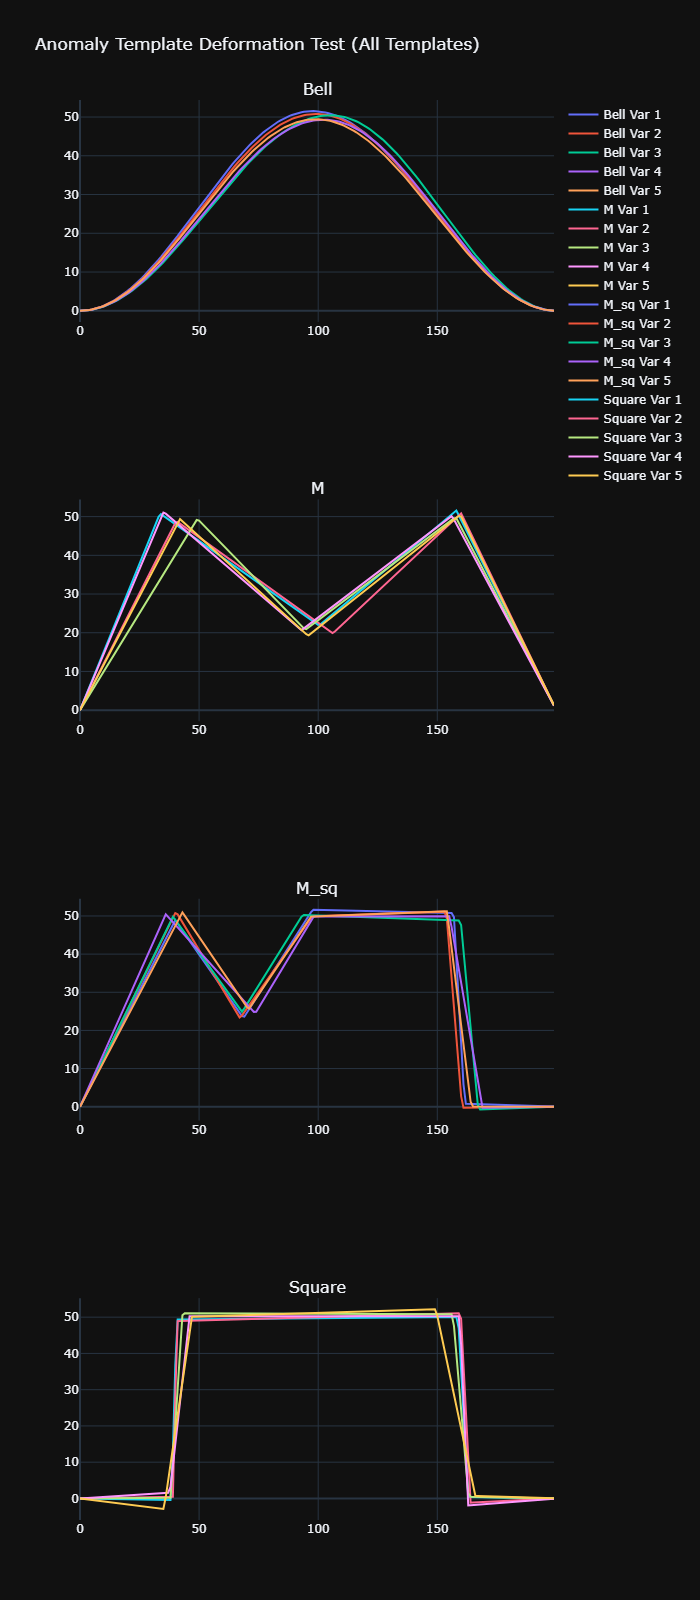
\includegraphics[width=\linewidth,height=0.85\textheight,keepaspectratio]{media/anomaly_template_deformation_test.png}
        \caption{Output of test\_generator\_deformation.py}
    \end{minipage}
\end{figure}

\subsection{Anomaly Template Creation}
Instead of relying on rigid pre-recorded dataset distributions, targeted geometric structures are freely defined as CSV blueprints in the \texttt{data-gen/anomalies/} folder.

\subsubsection{Configuration Blueprint (CSV Logic)}
A standard anomaly template requires 7 strict column definitions mapping normalized coordinates and behavioral constraints:
\\\texttt{time, value, t\_minus, t\_plus, v\_minus, v\_plus, interp}

\begin{itemize}
    \item \textbf{time \& value}: Normalized shape coordinates (scaling from 0.0 to 1.0). They define the key inflection points of the curve.
    \item \textbf{Deformation Multipliers (t\_minus, t\_plus, v\_minus, v\_plus)}: Define spatial jitter limits per control point. A value of \texttt{1.0} allows symmetric Gaussian distortion up to 100\% of the global variance parameter. A value of \texttt{0.0} locks the point rigidly in that direction.
    \item \textbf{interp (Interpolation Mode)}: Defines the mathematical connection between consecutive control points:
    \begin{itemize}
        \item \texttt{linear}: Simple linear interpolation between points.
        \item \texttt{exp\_up}: Concave-upward exponential growth (slow start, rapid finish), with curvature controlled by $\alpha = 3.0$.
        \item \texttt{exp\_down}: Concave-downward exponential curve (rapid start, slow finish), the complement of \texttt{exp\_up}.
        \item \texttt{bell}: Cosine envelope ($\frac{1}{2} - \frac{1}{2}\cos(\pi x)$), generating a smooth S-curve suitable for Gaussian-like bell shapes.
    \end{itemize}
\end{itemize}
